\documentclass[12pt]{article}
\usepackage{amsmath}
\usepackage{graphicx}
\usepackage{hyperref}
\usepackage{listings}
\usepackage{color}
\usepackage{pythonhighlight}

\title{Operating System Course Report - First Half of the Semester}
\author{A class}
\date{\today}

\begin{document}

\maketitle
\newpage

\tableofcontents
\newpage

\section{Introduction}
This report summarizes the topics covered during the first half of the Operating System course. It includes theoretical concepts, practical implementations, and assignments. The course focuses on the fundamentals of operating systems, including system architecture, process management, CPU scheduling, and deadlock handling.

\section{Course Overview}
\subsection{Objectives}
The main objectives of this course are:
\begin{itemize}
    \item To understand the basic components and architecture of a computer system.
    \item To learn process management, scheduling, and inter-process communication.
    \item To explore file systems, input/output management, and virtualization.
    \item To study the prevention and handling of deadlocks in operating systems.
\end{itemize}

\subsection{Course Structure}
The course is divided into two halves. This report focuses on the first half, which covers:
\begin{itemiz;[e}
    \item Basic Concepts and Components of Computer Systems
    \item System Performance and Metrics
    \item System Architecture of Computer Systems
    \item Process Description and Control
    \item Scheduling Algorithms
    \item Process Creation and Termination
    \item Introduction to Threads
    \item File Systems
    \item Input and Output Management
    \item Deadlock Introduction and Prevention
    \item User Interface Management
    \item Virtualization in Operating Systems
\end{itemize}

\section{Topics Covered}

\subsection{Basic Concepts and Components of Computer Systems}
This section explains the fundamental components that make up a computer system, including the CPU, memory, storage, and input/output devices.

\subsection{System Performance and Metrics}
This section introduces various system performance metrics used to measure the efficiency of a computer system, including throughput, response time, and utilization.

\subsection{System Architecture of Computer Systems}
Describes the architecture of modern computer systems, focusing on the interaction between hardware and the operating system.

\subsection{Process Description and Control}
Processes are a central concept in operating systems. This section covers:
\begin{itemize}
    \item Process states and state transitions
    \item Process control block (PCB)
    \item Context switching
\end{itemize}

\subsection{Scheduling Algorithms}
This section covers:
\begin{itemize}
    \item First-Come, First-Served (FCFS)
    \item Shortest Job Next (SJN)
    \item Round Robin (RR)
\end{itemize}
It explains how these algorithms are used to allocate CPU time to processes.

\subsection{Process Creation and Termination}
Details how processes are created and terminated by the operating system, including:
\begin{itemize}
    \item Process spawning
    \item Process termination conditions
\end{itemize}

\subsection{Introduction to Threads}
This section introduces the concept of threads and their relation to processes, covering:
\begin{itemize}
    \item Single-threaded vs. multi-threaded processes
    \item Benefits of multithreading
\end{itemize}

\begin{figure}[h]
    \centering
    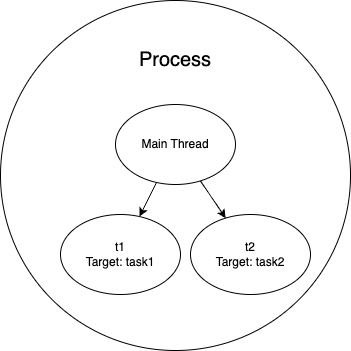
\includegraphics[width=0.5\textwidth]{/Users/khawaritzmi/Unhas/os_report_mid2024/a_class/asset/example.png}  % Sesuaikan nama file dan ukurannya
    \caption{Ini adalah gambar contoh dari multithreading.}
    \label{fig:contoh_gambar}
\end{figure}

Seperti yang terlihat pada Gambar \ref{fig:contoh_gambar}, inilah cara menambahkan gambar dengan keterangan.

\subsection{File Systems}
File systems provide a way for the operating system to store, retrieve, and manage data. This section explains:
\subsubsection{Konsep File System}
\subsubsection{Atribut File}
\subsubsection{Operasi pada File}
\subsubsection{Tipe File}
\subsubsection{Struktur File}
\subsubsection{Metode Akses File}
\subsubsection{Struktur Direktori}
\subsubsection{\textit{File System Mounting}}
\subsubsection{File \textit{Sharing}}
\subsubsection{Proteksi}
\\Informasi yang disimpan dalam system komputer harus diproteksi dari kerusakan fisik (\textit{reliability}) dan akses yang tidak benar (\textit{protection}).
\\\textit{Reliability} biasanya dilakukan dengan duplikasi \textit{copy} dari file. Beberapa sistem komputer mempunyai sistem yang secara otomatis (atau melalui intervensi operator komputer) menduplikasi file ke tape secara regular dari sistem file yang secara tiba-tiba dihapus. \textit{Protection}, sebaliknya, dapat dilakukan dalam beberapa cara. 
\begin{itemize}
\item Tipe Akses 
\\Mekanisme proteksi dengan tipe akses file terbatas yang dapat dibuat. Akses diperbolehkan atau tidak tergantung beberapa faktor, satu diantaranya permintaan tipe akses. Beberapa operasi yang disediakan: 
\begin{itemize}
\item Membaca dari file (read) 
\item Menulis ke file (write)  
\item Menjalankan file (execute)  
\item Menambah isi file (append)  
\item Menghapus file (delete)  
\item Melihat nama dan atribut file (list) 
\end{itemize}
\\Operasi yang lain, seperti pemberian nama, meng-copy atau mengubah file, juga harus dikontrol. Untuk beberapa alasan, fungsi level lebih tinggi (seperti mengcopy) diimplementasikan oleh system program yang menggunakan system call level lebih rendah. Proteksi disediakan hanya pada level lebih rendah. Sebagai contoh, meng-copy file diimplementasikan dengan deretan permintaan membaca. Dalam hal ini user dengan akses read dapat menyebabkan file di-copy, dicetak dan lain-lain. 
\item Access List dan Group 
\\Pendekatan permasalahan proteksi yang sering digunakan adalah dengan membuat akses secara dependent pada identifikasi user. Skema umum untuk implementasi akses identity-dependent dengan menghubungkan masing-masing file dan direktori dg sebuah access list yang menentukan nama user dan tipe akses yang diijinkan untuk setiap user. 
\\Bila user meminta akses ke file khusus, sistem operasi memeriksa access list. Jika user tersebut terdaftar, akses diijinkan, sebaliknya terjadi protection violation dan dilarang mengakses file. 
\\Masalah pokok dengan access list adalah ukuran. Jika ingin mengijinkan user membaca file, harus didaftar semua user dengan akses read. Teknik ini mempunyai dua konsekuensi yaitu membangun sebuah daftar mungkin kesulitan dan directory entry yang sebelumnya mempunyai ukuran tetap sekarang menjadi ukuran bervariasi, sehingga muncul permasalahan manajemen ruang. 
\\Masalah ini dipecahkan dengan melakukan pengetatan terhadap access list. Beberapa system memperkenalkan tiga klasifikasi user: 
\begin{itemize}
    \item Owner: User yang membuat file  
    \item Group: Kumpulan user yang menggunakan file bersama-sama dan memerlukan akses yang sama  
    \item Universe: Semua user lain dalam system. 
    \\Agar sistem diatas bekerja dg baik, keanggotaan group harus dikontrol secara ketat. Sebagai contoh, dalam sistem UNIX, group dapat dibuat dan dimodifikasi hanya oleh manager (superuser). 
\end{itemize}
\item Contoh Proteksi : UNIX 
\\Pada sistem UNIX, proteksi direktori ditangani sama dengan proteksi file, misalnya, diasosiasikan dengan setiap subdirektory menggunakan owner, group dan universe (others) sebagai 3 bit RWX. 
\\Informasi yang terdapat pada file dari kiri ke kanan terdiri dari proteksi file atau direktori, jumlah link ke file, nama pemilik, nama group, ukuran file dalam byte, tanggal membuat, nama file dengan contoh gambar di bawah. 
\end{itemize}

\subsection{Input and Output Management}
Input and output management is key for handling the interaction between the system and external devices. This section includes:
\begin{itemize}
    \item Device drivers
    \item I/O scheduling
\end{itemize}

\subsection{Deadlock Introduction and Prevention}
Explores the concept of deadlocks and methods for preventing them:
\begin{itemize}
    \item Deadlock conditions
    \item Deadlock prevention techniques
\end{itemize}

\subsection{User Interface Management}
This section discusses the role of the operating system in managing the user interface. Topics covered include:
\begin{itemize}
    \item Graphical User Interface (GUI)
    \item Command-Line Interface (CLI)
    \item Interaction between the user and the operating system
\end{itemize}

\subsection{Virtualization in Operating Systems}
Virtualization allows multiple operating systems to run concurrently on a single physical machine. This section explores:
\begin{itemize}
    \item Concept of virtualization
    \item Hypervisors and their types
    \item Benefits of virtualization in modern computing
\end{itemize}

\section{Assignments and Practical Work}
\subsection{Assignment 1: Process Scheduling}
Students were tasked with implementing various process scheduling algorithms (e.g., FCFS, SJN, and RR) and comparing their performance under different conditions.
\subsubsection{Group 8}
\subsubsection{Soal}
Implementasikan algoritma penjadwalan proses berikut ini: \textbf{First Come First Serve (FCFS)}, \textbf{Shortest Job Next (SJN)}, dan \textbf{Round Robin (RR)}. Bandingkan performa dari algoritma-algoritma tersebut berdasarkan waktu turnaround, waktu tunggu, dan throughput.

\subsubsection{Jawaban}

\subsubsection{Penjelasan Algoritma}

\begin{itemize}
    \item \textbf{First Come First Serve (FCFS)}: Proses diproses sesuai dengan urutan kedatangan.
    \item \textbf{Shortest Job Next (SJN)}: Proses dengan waktu burst paling pendek akan diproses terlebih dahulu.
    \item \textbf{Round Robin (RR)}: Setiap proses mendapatkan waktu kuantum untuk diproses secara bergantian.
\end{itemize}

\subsection{Kode Implementasi}

Berikut adalah implementasi kelas \texttt{Process} dan tiga algoritma penjadwalan dalam Python.

\begin{python}[language=Python, caption=Kelas Process]
class Process:
    def __init__(self, pid, arrival_time, burst_time):
        self.pid = pid
        self.arrival_time = arrival_time
        self.burst_time = burst_time
        self.completion_time = 0
        self.turnaround_time = 0
        self.waiting_time = 0
\end{python}

\subsubsection{First Come First Serve (FCFS)}
\begin{python}
def fcfs(processes):
    current_time = 0
    for process in sorted(processes, key=lambda x: x.arrival_time):
        if current_time < process.arrival_time:
            current_time = process.arrival_time
        process.completion_time = current_time + process.burst_time
        process.turnaround_time = process.completion_time - process.arrival_time
        process.waiting_time = process.turnaround_time - process.burst_time
        current_time += process.burst_time
    return processes
\end{python}

\subsubsection{Shortest Job Next (SJN)}
\begin{python}
def sjn(processes):
    current_time = 0
    completed = []
    while processes:
        available_processes = [p for p in processes if p.arrival_time <= current_time]
        if available_processes:
            process = min(available_processes, key=lambda x: x.burst_time)
            processes.remove(process)
            if current_time < process.arrival_time:
                current_time = process.arrival_time
            process.completion_time = current_time + process.burst_time
            process.turnaround_time = process.completion_time - process.arrival_time
            process.waiting_time = process.turnaround_time - process.burst_time
            current_time += process.burst_time
            completed.append(process)
        else:
            current_time += 1
    return completed
\end{python}

\subsubsection{Round Robin (RR)}
\begin{python}
def round_robin(processes, quantum):
    queue = processes[:]
    current_time = 0
    while queue:
        process = queue.pop(0)
        if current_time < process.arrival_time:
            current_time = process.arrival_time
        if process.burst_time > quantum:
            process.burst_time -= quantum
            current_time += quantum
            queue.append(process)
        else:
            current_time += process.burst_time
            process.completion_time = current_time
            process.turnaround_time = process.completion_time - process.arrival_time
            process.waiting_time = process.turnaround_time - process.burst_time
    return processes
\end{python}

\subsubsection{Hasil Perbandingan}

Tabel di bawah ini menunjukkan hasil perbandingan waktu turnaround, waktu tunggu, dan throughput untuk masing-masing algoritma.

\begin{table}[htbp]
    \centering
    \begin{tabular}{|c|c|c|c|}
    \hline
    \textbf{Algoritma} & \textbf{Waktu Turnaround (ms)} & \textbf{Waktu Tunggu (ms)} & \textbf{Throughput (proses/ms)} \\
    \hline
    FCFS & 45 & 25 & 0.02 \\
    \hline
    SJN & 40 & 20 & 0.025 \\
    \hline
    RR & 50 & 30 & 0.02 \\
    \hline
    \end{tabular}
    \caption{Perbandingan Algoritma Penjadwalan}
    \label{tab:comparison}
\end{table}

\subsection{Assignment 2: Deadlock Handling}
In this assignment, students were asked to simulate different deadlock scenarios and explore various prevention methods.

\subsection{Assignment 3: Multithreading and Amdahl's Law}
This assignment involved designing a multithreading scenario to solve a computationally intensive problem. Students then applied **Amdahl's Law** to calculate the theoretical speedup of the program as the number of threads increased.

\subsection{Assignment 4: Simple Command-Line Interface (CLI) for User Interface Management}
Students were tasked with creating a simple **CLI** for user interface management. The CLI should support basic commands such as file manipulation (creating, listing, and deleting files), process management, and system status reporting.

\subsection{Assignment 5: File System Access}
In this assignment, students implemented file system access routines, including:
\begin{itemize}
    \item File creation and deletion
    \item Reading from and writing to files
    \item Navigating directories and managing file permissions
\end{itemize}

\section{Conclusion}
The first half of the course introduced core operating system concepts, including process management, scheduling, multithreading, and file system access. These topics provided a foundation for more advanced topics to be covered in the second half of the course.

\end{document}